\documentclass[a4paper]{article}     
\usepackage{amsfonts}
\usepackage{amsmath}
\usepackage{amssymb}
\usepackage{graphicx}
\newcommand{\dint}{\displaystyle\int}

\begin{document}

\noindent \large Auteur: Michaël Francken \\
\noindent \large Studierichting: Informatica\\
\noindent \large Oefeningenreeks 5D nr. 4.2\\

\medskip

\normalsize

$y=-2x^2+6x$\\

$y=x^2$\\

$-2x^2+6x=x^2$\\

$=-3x^2(x-2)$\\

nullpunten zijn $0$ en $2$\\

voor $x=1$\\

$y_1=-2(1)^2+6(1)=4$\\

$y_2=1^2=1$\\

$\Rightarrow y_1>y_2$\\

$\displaystyle\int^2_0\left(-3x^2+6x\right)$\\

$=\left[-x^3+3x^2\right]^2_0$\\

$=\left(-(2)^3+3(2)^2\right)-0$\\

$=-8+12=4$\\

\begin{figure}[h]
\centering
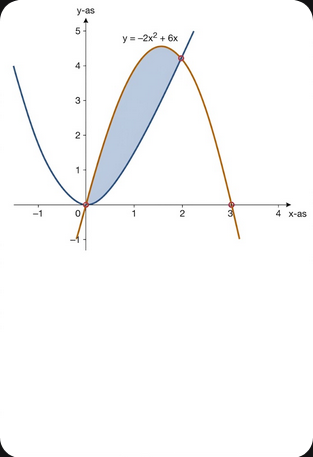
\includegraphics[width=5cm]{5D-4.2-michael.francken.INF.png}
\end{figure}

\begin{thebibliography}{999}
%\bibitem{a} Referentie
\end{thebibliography}
\end{document} 
